% !TEX root = Hauptdatei.tex
\section{Implementierung in QtCreator}\label{hauptabschnitt_2}

Diese Kapitel beschäftigt sich damit, wie eine \ac{HMI} in Qt im Hinblick auf das Architektur-Konzept umgesetzt werden kann.\\

\subsection{Simulation der Fahrzeugdaten}
Normalerweise erhält das \ac{HMI} die Daten des Fahrzeugs vom \ac{KSS} über \ac{CAN}. Für das Proof-of-Concept wird eine Simulation der Daten mit einem UI-Window von Qt realisiert. Qt ermöglicht mit dem Qt Designer die Entwicklung von Formsanwendungen. Die Formsanwendung soll als Dashboard dienen, in dem verschieden Daten zur Laufzeit manipuliert werden können (z.B. Geschwindigkeit, Drehzahl, etc.).\\

%quelle https://doc.qt.io/qt-5/designer-to-know.html
\begin{figure}[htb]
	\centering
	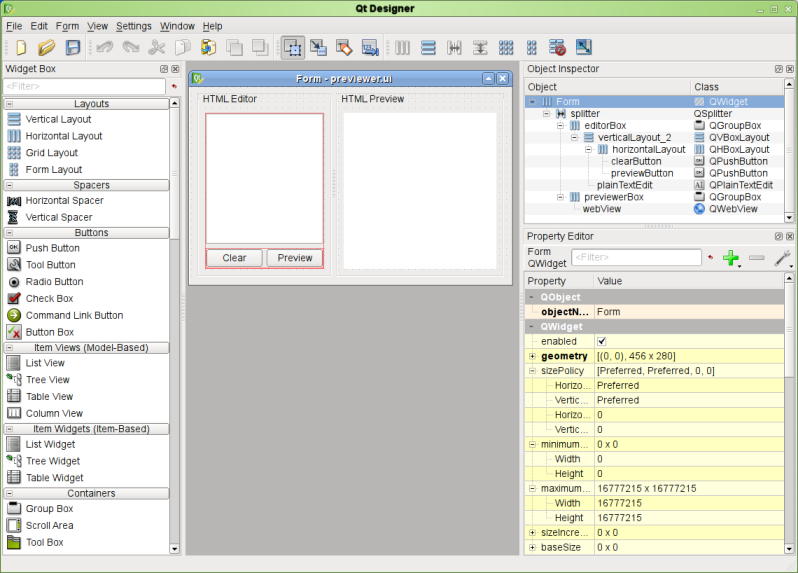
\includegraphics[width=\textwidth]{img/5_implementierung/qt_designer}
	\caption[Übersicht des QtDesigners]{Übersicht des QtDesigners \cite{qt_designer}}
	\label{fig:qt_designer}
\end{figure}

Abbildung \ref{fig:qt_designer} zeigt eine Übersicht des Qt Designer. Links ist eine Auswahl der verschiedenen Forms-Elemente zu sehen. Diese können per Drag and Drop in das Fenster in der Mitte gezogen werden. Qt erstellt für diese Fenster jeweils eine Header-Datei und Quell-Datei, diese Dateien ermöglichen das Einlesen und die Verarbeitung der Werte in C++.\\

Für das Proof-of-Concept wird ein Dashboard implementiert. Das Dashboard besteht aus verschiedenen Slidern, Combo Boxen, Buttons und anderen Formselementen. Abbildung \ref{fig:ui_window} zeigt eine Version dieses Fensters.\\

\begin{figure}[htb]
	\centering
	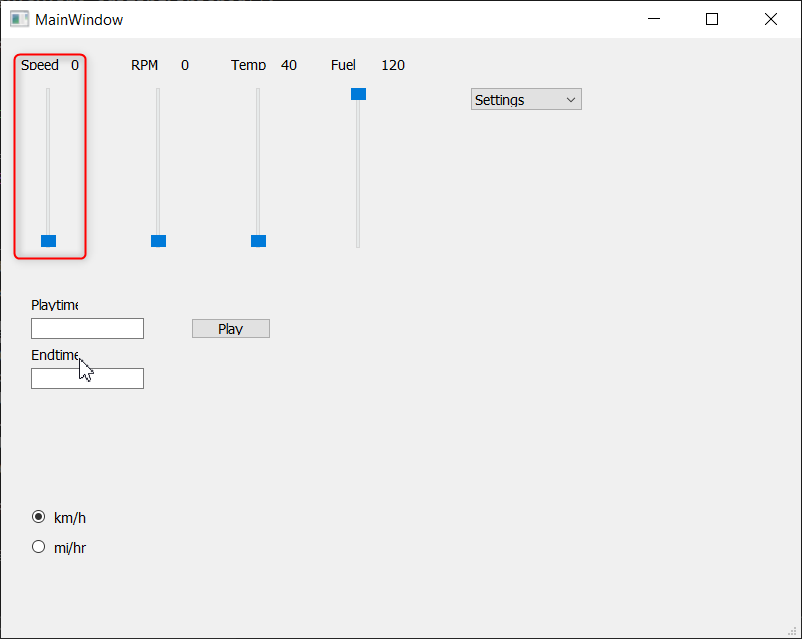
\includegraphics[width=\textwidth]{img/5_implementierung/ui_window}
	\caption[Aufbau des UI Formularfensters]{Aufbau des UI Formularfensters. Dieses ermöglicht im Folgenden die Eingabe der Fahrzeugdaten, welche im realen Fahrzeug vom Steuergerät gesendet werden.}
	\label{fig:ui_window}
\end{figure}

Jedes Formselement bietet verschiedene Funktionen um die Werte auszulesen. Der Wert eines Sliders kann z.B. über die Funktion \textit{on\_speedSlider\_valueChanged(int value)} ausgelesen werden. Diese Funktion wird aufgerufen, sobald sich der Wert des Sliders verändert. Der Parameter \textit{value} beinhaltet dabei den aktuellen Wert.\\

\subsection{Implementierung des Models}
Das Model wird als eigenständige Klasse umgesetzt. Wie im Architektur-Konzept beschrieben, besteht das Model aus mehreren, austauschbaren Klassen. So existiert beispielsweise jeweils für die Geschwindigkeits-, Drehzahl-, Temperatur- und Tankanzeige eine eigene Klasse. Diese Klassen werden im Model zusammengeführt. Das Model ist damit ein Fassadenmuster und bietet ein Interface zu den einzelnen Klassen.\\

\begin{figure}[htb]
	\centering
	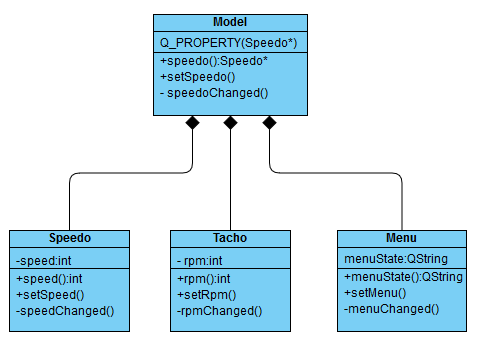
\includegraphics[width=10cm]{img/5_implementierung/implement_model}
	\caption[UML-Klassendiagramm des Models]{UML-Klassendiagramm des Models mit Beispiel-Modulen}
	\label{fig:implement_model}
\end{figure}

Abbildung \ref{fig:implement_model} zeigt ein beispielhaftes Klassendiagramm. Das Diagramm zeigt wie die Speedo-Klasse im Model implementiert ist und die Implementierung der Speedo-, Tacho- und Menu-Klasse. Die Speedo-Klasse ist für die Geschwindigkeit des Fahrzeugs verantwortlich. Jede weitere Klasse ist ähnlich aufgebaut, mit einer Set-, Get- und Signalfunktion. Mit der Set-Funktion wird mit Signals und Slots die Geschwindigkeit eingelesen. Die Signalfunktion zeigt an, ob der Wert geändert wurde. Bei einer Wertänderung kann der Wert dann mit der Get-Funktion ausgelesen werden.\\

Die Klassen innerhalb des Models werden über das Signals und Slots System von Qt mit Daten versorgt. Das Signals und Slots System entspricht der Umsetzung des Beobachter-Musters. Mit Signals und Slots können Daten klassenübergreifend ausgetauscht werden, ohne dabei die Klassen zu stark zu koppeln. Sobald ein Wert in der Formsanwendung verändert wird, wird ein Signal emittiert. Das Emittieren des Signals führt dazu, dass eine Set-Funktion in der Zielklasse ausgeführt wird. Dadurch ist der veränderte Wert in der Zielklasse verwendbar. Mit dieser Vorgehensweise werden alle Daten aus der Formsanwendung an die verschiedenen Klassen im Model verteilt.\\

Vom Model aus müssen die Daten in ähnlicher Form an den Controller bzw. die View verteilt werden. Bei der Verteilung an die View wird zusätzlich noch das Property System von Qt benötigt. Das Property System ermöglicht, dass die View die Daten aus dem Model auslesen und verarbeiten kann. %Property System genauer erklären?

Abbildung \ref{fig:uml_sequenz} zeigt ein UML-Sequenzdiagramm mit beispielhaften Signalen. Der Großteil der Daten kann direkt vom Model an die View gesendet werden. Das gilt für alle fahrzeugbezogenen Daten. Benutzereingaben werden hingegen zunächst vom Controller verarbeitet. Im Controller wird geprüft ob es notwendig ist in einen anderen Zustand zu wechseln, z.B. in ein anderes Menü springen. Anschließend werden die Daten ebenfalls an die View weitergegeben um beispielsweise das Menü korrekt darzustellen.\\

\begin{figure}[htb]
	\centering
	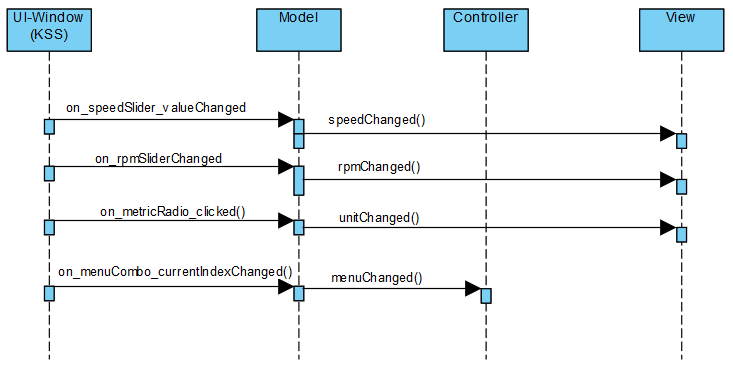
\includegraphics[width=\textwidth]{img/5_implementierung/uml_sequenz}
	\caption{Sequenzdiagramm mit beispielhaften Signalverläufen}
	\label{fig:uml_sequenz}
\end{figure}

\subsection{Implementierung des Controllers}
Für die Umsetzung des Controllers gibt es zwei Möglichkeiten. Der Controller kann als eigene Klasse implementiert werden. Qt bietet dafür ein Zustandsautomaten-Frame"=work an. Für den Controller wird vor allem die QState-Klasse und die verschiedenen Transitions benötigt. Damit könnte der Controller wie im Architektur-Konzept vorgesehen umgesetzt werden. Dadurch sind alle Zustände und Zustandsübergänge zentral an einem Ort. Der Entwicklungsaufwand ist dadurch etwas höher.\\

Im Gegensatz dazu könnten alle Zustände auch dezentral in den einzelnen QML-Dateien angelegt werden. In QML existiert dazu die State Funktion. Diese Funktion ermöglicht es verschieden Zustände zu erstellen. In jedem Zustand kann das Erscheinungsbild der QML-Komponente verändert werden. Der Zustand lässt sich zum einen über Wenn-Bedingung ändern, zum anderen kann der Zustand direkt über die Eigenschaft \textit{state} gewechselt werden. Diese Vorgehensweise erspart die Erstellung einer eigenen Klasse für den Controller, allerdings leidet darunter die Übersichtlichkeit aber einer bestimmten Menge von Zuständen.\\

\subsection{Implementierung der View}
Die View hängt stark vom verwendeten Framework ab. Daher ist im Architektur-Konzept kein UML-Diagramm dafür vorgesehen. Die Implementierung der View mit Qt ist zum größten Teil bereits durch die Umsetzung der Use Cases in den vorherigen Kapiteln abgedeckt. Allerdings wurde die View im Qt Design Studio umgesetzt, die View muss daher noch in das QtCreator Projekt implementiert werden.\\

Um ein Qt Design Studio Projekt in ein QtCreator Projekt zu Konvertieren reicht es der Anleitung in der Dokumentation von Qt zu folgen.\\

Die View ist damit in das QtCreator Projekt eingebunden. Anschließend muss eine Verbindung zum Model hergestellt werden. Zunächst muss QML mitgeteilt werden, dass das Model existiert. Mit der Funktion \textit{setContextProperty()} kann in QML zumindest auf das Model zugegriffen werden. Damit auch ein Zugriff auf die Unterklassen (Speedo, Tacho, etc.) möglich ist, muss mit der Funktion \textit{qRegisterMetaType()} jede Unterklasse registriert werden. Dadurch kann die View auf die Werte im Model zugreifen. Der Geschwindigkeitswert kann dann mit \textit{Model.speedo.speed} ausgelesen werden.\\